\begin{figure}[hbt!]
  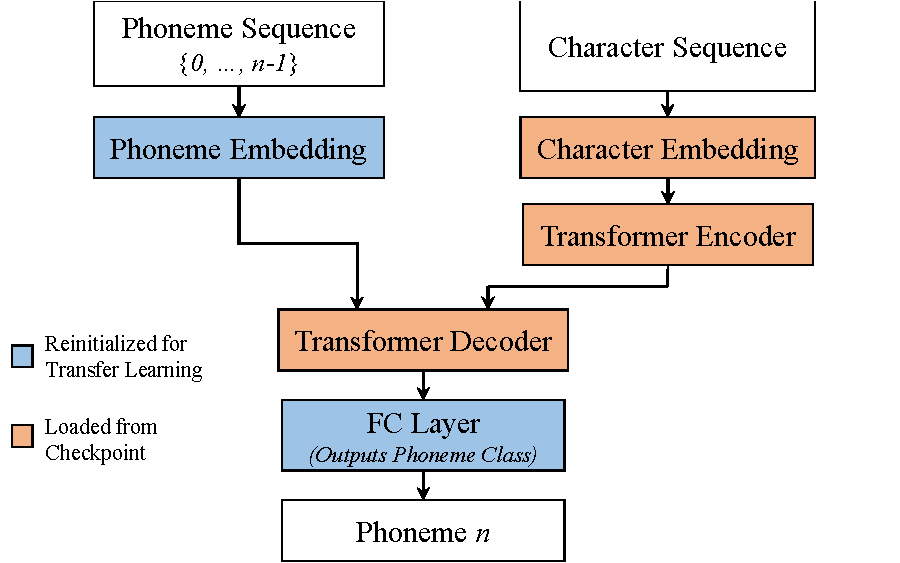
\includegraphics[width=\linewidth]{figures/g2p_model_2.pdf}
   \caption{Diagram of the transformer model used, highlighting the layers that were replaced for transfer-learning and the layers that were kept the same from the pretrained model checkpoint.}
   \label{fig:g2pmodel}
\end{figure}
\begin{table}[h!]
\caption{Transformer Model hyper-parameters}
 \label{tab:table1}
  \begin{center}
\begin{tabular}{rc} 
\toprule
\textbf{Hyper Parameter} & \textbf{Value}  \\ 
\toprule
Encoder Layers                               & 3               \\
Decoder Layers                               & 3               \\
Hidden Width                                 & 256             \\
Position-wise Feedforward Width              & 512             \\
Attention Heads                              & 8               \\
Dropout Probability                          & 0.1             \\
Sequence Length                              & 240             \\
Normalization                                & Layer Norm      \\
\toprule
\end{tabular}
  \end{center}
\end{table}
\section{Model}
The Transformer architecture is a successful generic sequence-to-sequence model designed for neural machine translation. As G2P can be seen as a translation problem, translating graphemes to their phonetic counterparts, the Transformer architecture can be applied to G2P problems ~\cite{yolchuyeva2020transformer,vesik2020model,vesik2020model}. We use the Transformer architecture, ~\cite{Vaswani2017AttentionIA}, for our experiments, also see Figure~\ref{fig:g2pmodel}. We use the hyper-parameters specified in Table~\ref{tab:table1} for all experiments. During training, the hyper parameters are fixed across all models as seen in Table ~\ref{tab:table2}. The resulting Transformer model has $4.1$M parameters.
% 
% 
We train our Transformer models in the following setup(s):
\begin{enumerate}
    \item Pre-train the Transformer model using our CMUDict American English dialect data for 100 epochs, and save the model with the best validation loss.
    \item Train the Transformer model from scratch on both dialects, varying the dictionary size across [1K, 3K, 5K, 10K] words. We train the model for 50 epochs and select the model with the best validation loss for testing.
    \item Load the pre-trained Transformer model from setup 1. Then replace the embedding and output FC layers in the Decoder with new layers of the appropriate size for the differing output phoneme sets (see Figure~\ref{fig:g2pmodel} for details), dependent on dialect.  Finally, we fine-tune this model for 25 epochs on the same dialect and training dictionary size combinations as in setup two, again selecting the model with the best validation loss at the end of training.
\end{enumerate}

\begin{table}[h!]
 \caption{Training hyper-parameters}
 \label{tab:table2}
  \begin{center}
\begin{tabular}{rc} 
\toprule
\textbf{Hyper Parameter} & \textbf{Value}  \\ 
\toprule
Learning Rate            & 0.0005          \\
Batch Size               & 128             \\
Gradient Norm Clipping   & 1.0             \\
Initialization           & Xavier Uniform  \\
Optimizer                & Adam            \\
Random Seed              & 1234            \\
\toprule
\end{tabular}
    % \begin{tabular}{c|c} % <-- Alignments: 1st column left, 2nd middle and 3rd right, with vertical lines in between
    %     \hline
    %     \textbf{Hyper Parameter} & \textbf{Value}\\
    %     \hline
    %     Learning Rate & 0.0005 \\
    %     Batch Size & 128 \\
    %     Gradient Norm Clipping & 1.0 \\
    %     Initialization & Xavier Uniform (PyTorch) \\
    %     Optimizer & Adam \\
    %     Random Seed & 1234 \\
    %     \hline
    % \end{tabular}
  \end{center}
\end{table}